\chapter{Material and Methods}
\section{Invitrodb}
The most recent release of the ToxCast's (Toxicity Forecaster) database, referred to as \href{https://cfpub.epa.gov/si/si_public_record_Report.cfm?dirEntryId=355484&Lab=CCTE}{invitroDBv3.5}, serves as a source of an extensive collection of high-throughput screening (HTS) targeted bioactivity data. This database encompasses information on a total of 9541 compounds, selectively screened across 2205 assay endpoints. This resource originated from the collaboration of two prominent institutions: the United States Environmental Protection Agency (\href{https://www.epa.gov/chemical-research/exploring-toxcast-data}{EPA}) through its ToxCast program and the National Institutes of Health (\href{https://ntp.niehs.nih.gov/whatwestudy/tox21}{NIH}) via the Tox21 initiative. Incorporating data collected from diverse research laboratories, this relational database is openly accessible to the public and can be downloaded directly from the official ToxCast website.


\subsection{Data Overview}
\subsubsection{Presence Matrix}
Consider a collection of $m$ assay endpoints, denoted by $A = \{a_1, a_2, \dots, a_m\}$ and a set of $n$ compounds represented as $C = \{c_1, c_2, \dots, c_n\}$.
To facilitate data comprehension, we introduce a \emph{presence matrix} $P \in {\{0, 1\}}^{m \times n}$. Rows, indexed by $i$, represent assay endpoints $a_i$, while columns, indexed by $j$, denote presence (1) or absence (0) of compound $c_j$ in those endpoints. Matrix $P$ is sparse due to the selective testing of compounds across different assay endpoints. A compound is considered present in an assay endpoint if it has undergone testing and a corresponding concentration-response series is available.
See Figure~\ref{fig:presence_matrix_all} for a visual of the \emph{presence matrix} $P$ covering all assay endpoints and compounds in \textit{invitroDBv3.5}. 

\begin{figure}[h]  % Placement options: h (here), t (top), b (bottom), p (page)
    \centering
    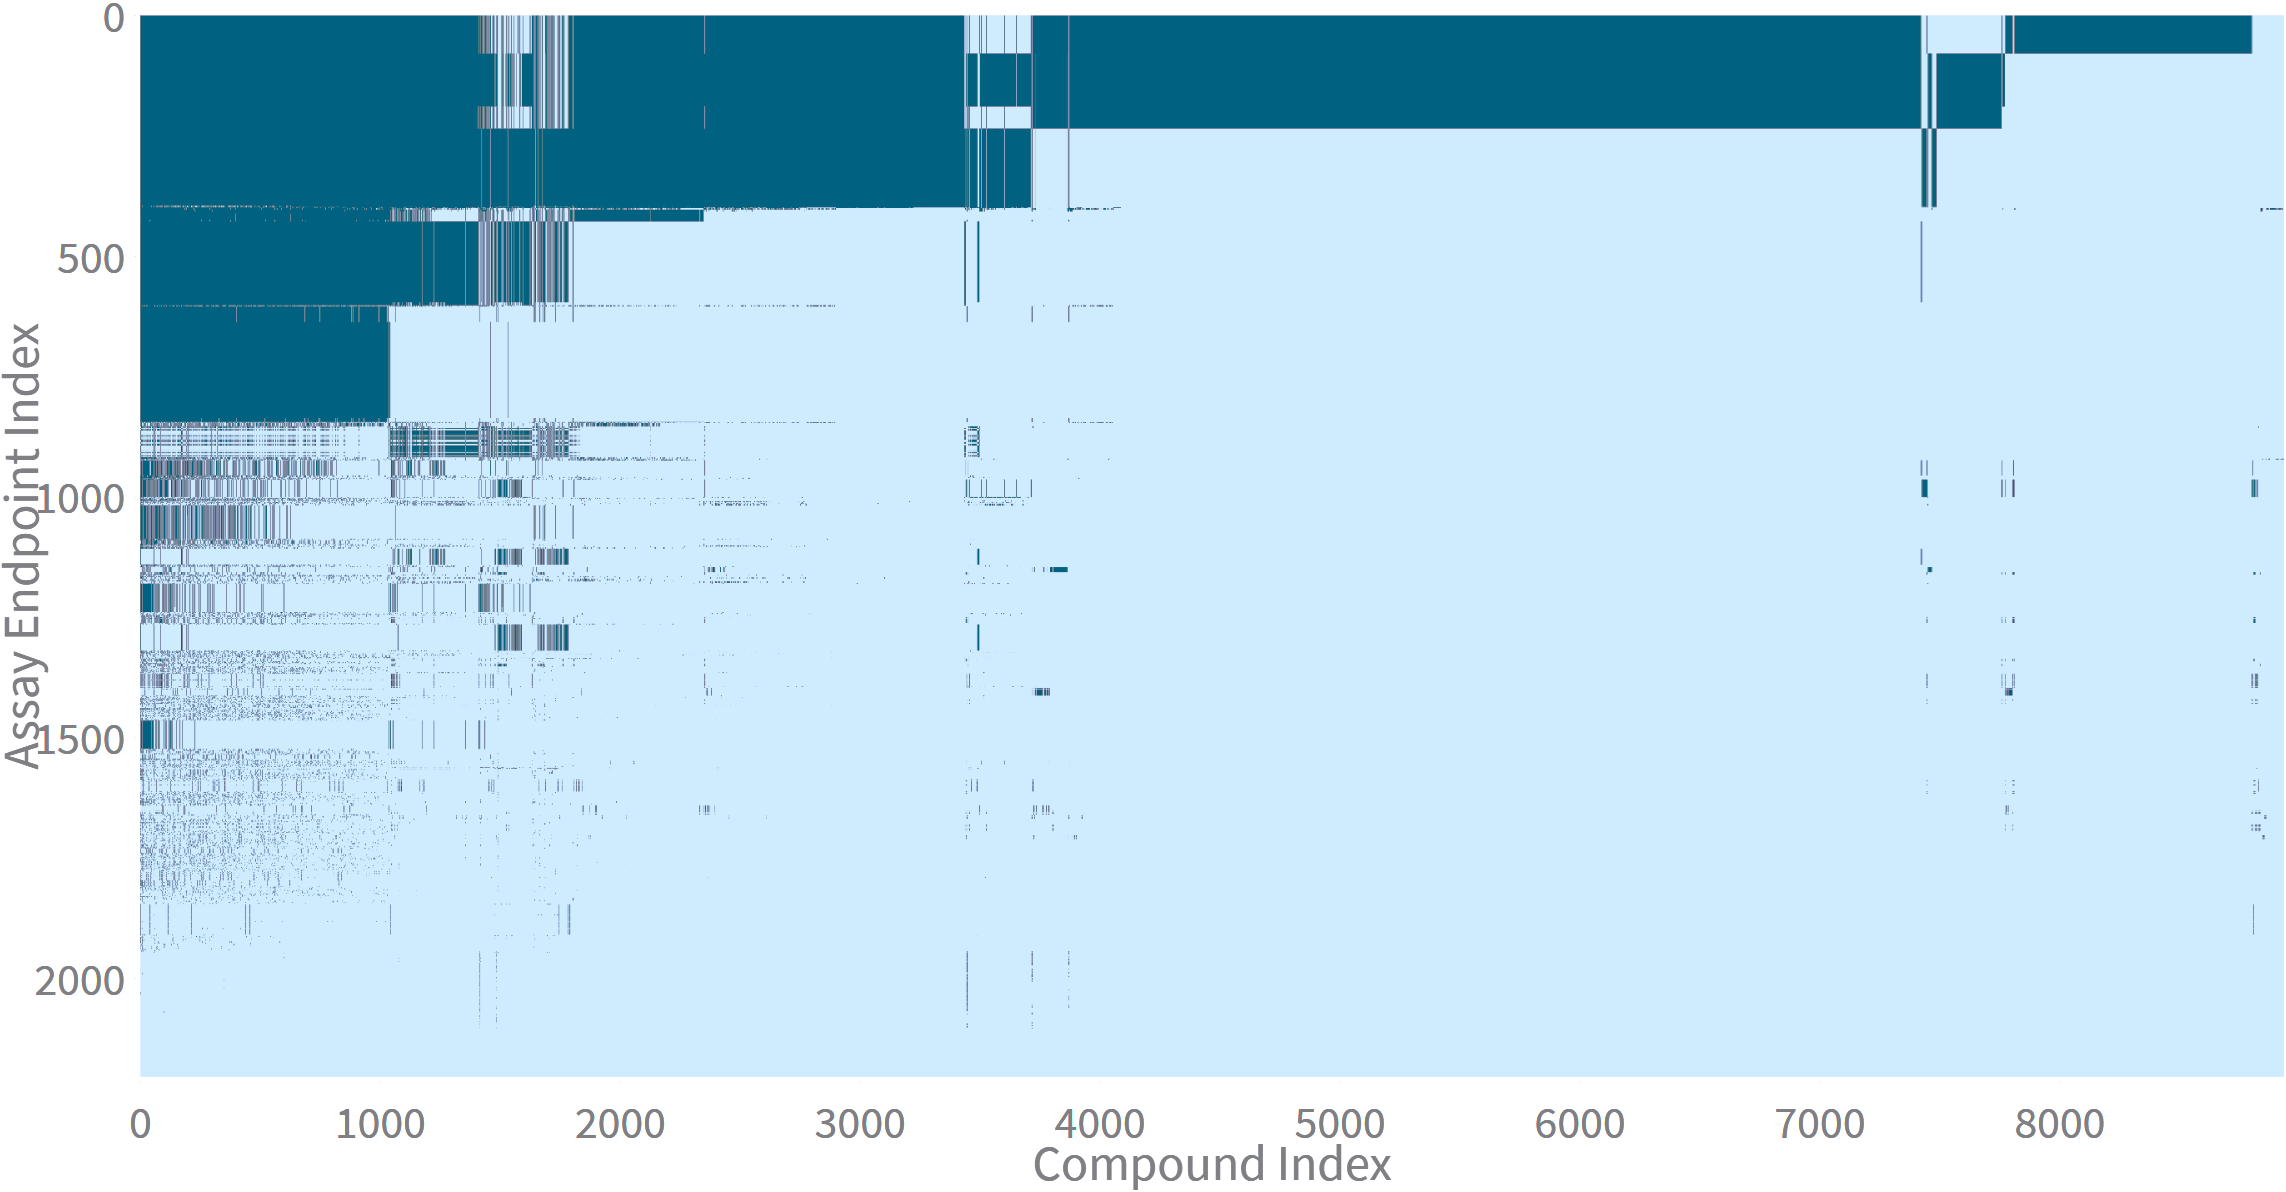
\includegraphics[width=1.0\textwidth]{figures/presence_matrix_all.png}  
    \caption{The \emph{presence matrix} $P$ covering all assay endpoints and compounds available in \textit{invitroDBv3.5} with $m = \num{2205}$ assay endpoints and $n = \num{9541}$ compounds. The presence matrix is organized by sorting it based on the number of compounds present in each assay endpoint and the compounds are arranged in descending order of their presence frequency. The total count, where $P_{ij} = 1$, indicates the availability of \num{3342377} concentration-response series for downstream analysis.}
~\label{fig:presence_matrix_all} 
\end{figure}

\subsubsection{Subsetting data}
We exclusively consider assay endpoints that have been tested with a minimum of $\num{2000}$ compounds. This criterion ensures the availability of sufficient data for the training of a machine learning model. Refer to Figure~\ref{fig:presence_matrix_subset} for a visual representation of the \emph{presence matrix} $P$, which now encompasses only the resulting subset of all assay endpoints within \textit{invitroDBv3.5}. From now on, we will call this specific subset the data that we will be focusing on for this thesis. 


\begin{figure}[h]  % Placement options: h (here), t (top), b (bottom), p (page)
    \centering
    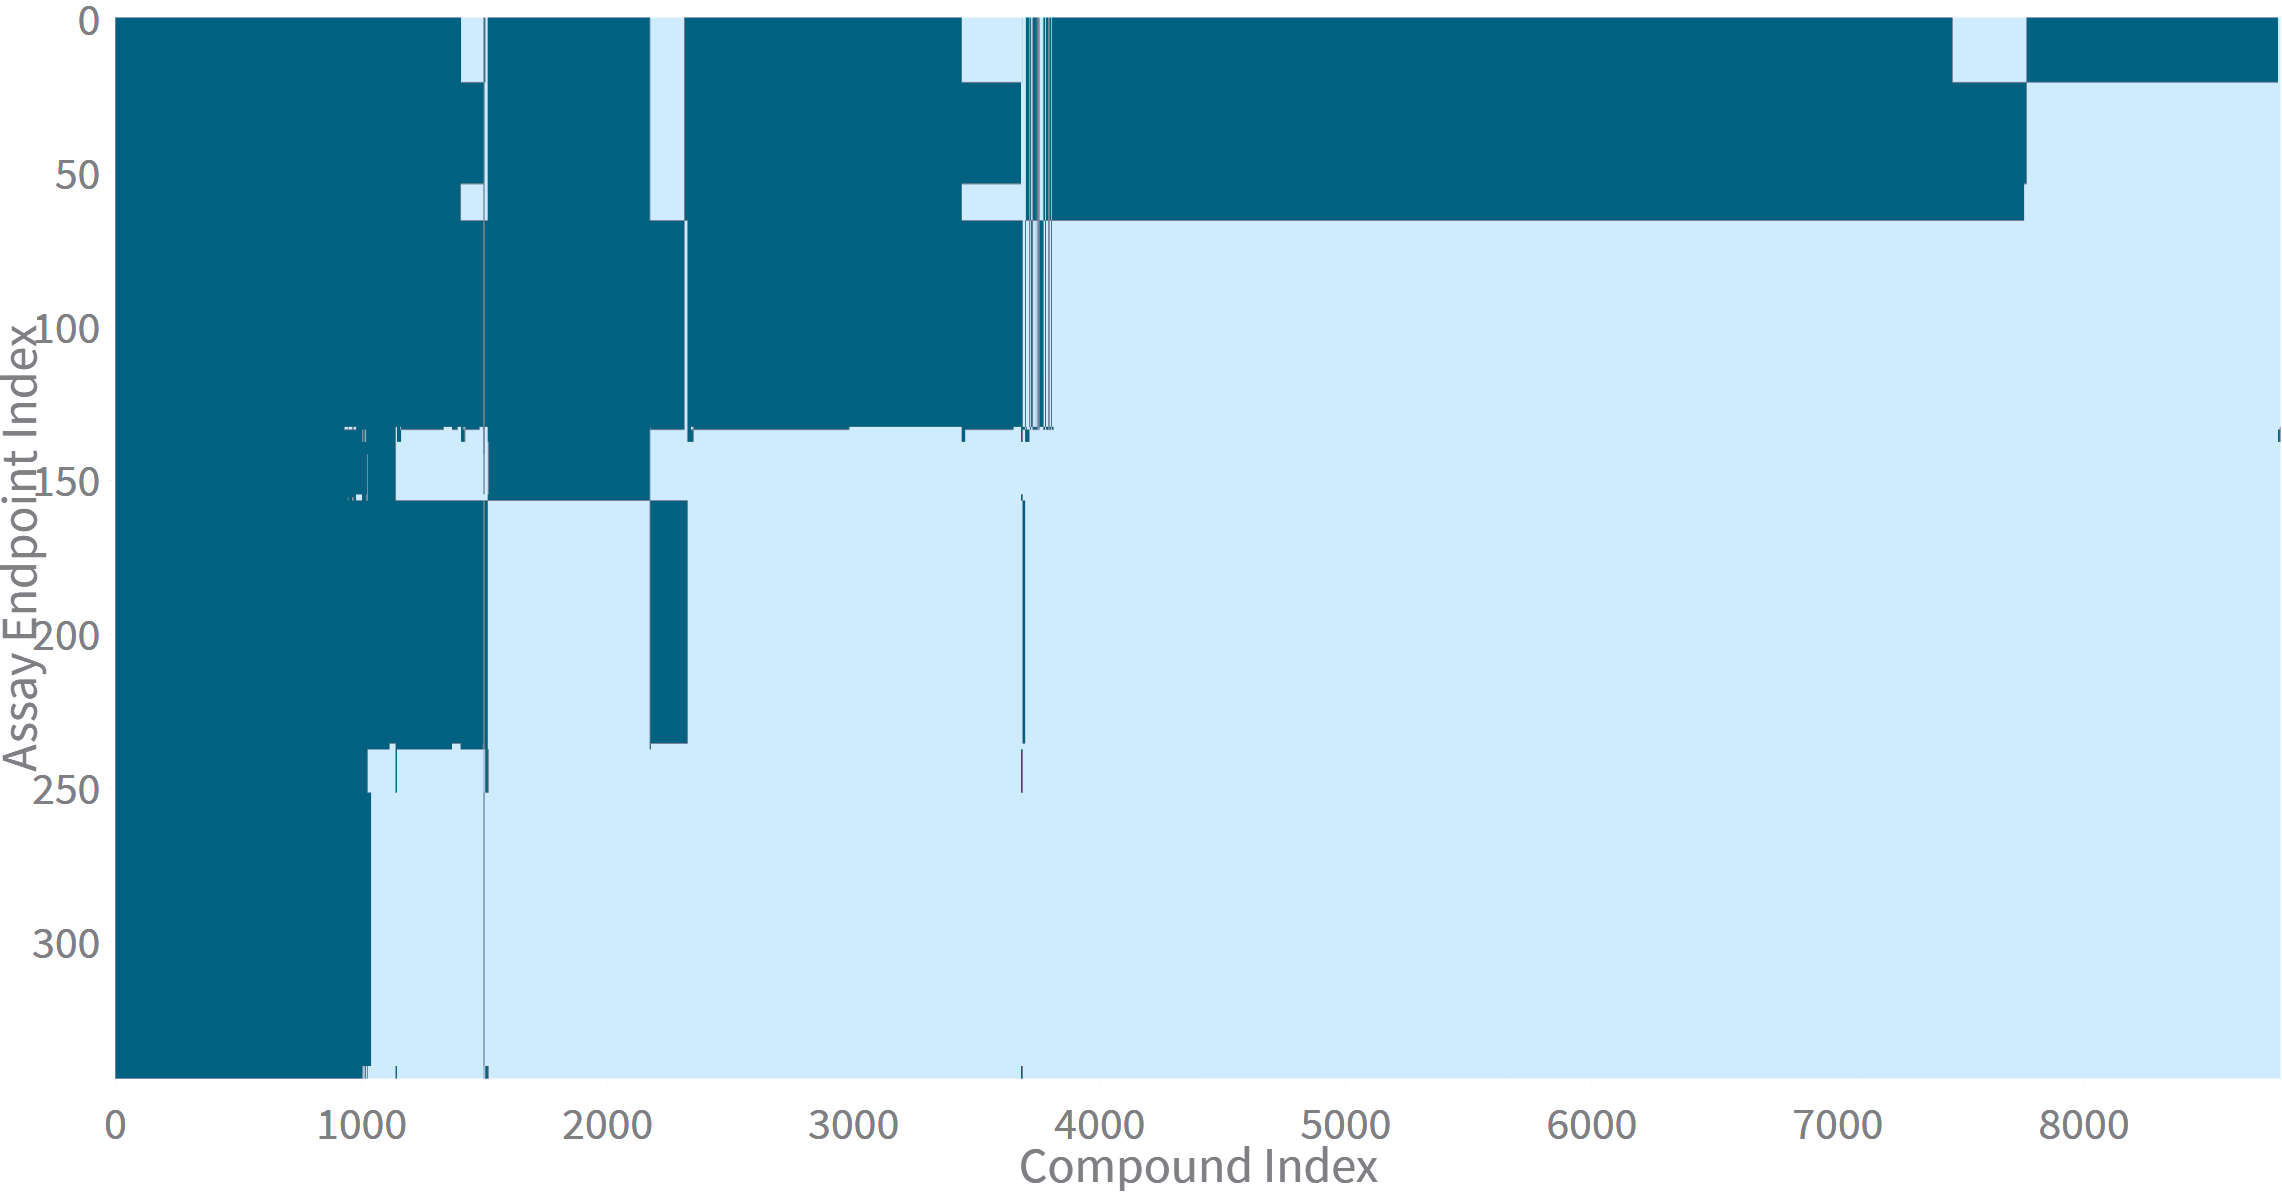
\includegraphics[width=1.0\textwidth]{figures/presence_matrix_subset.png}  
    \caption{The \emph{presence matrix} $P$ covering only the subset of all of assay endpoints available in \textit{invitroDBv3.5}, considered for this thesis, encompassing $m = \num{271}$ assay endpoints and $n = \num{9456}$ compounds. The total count, where $P_{ij} = 1$, indicates the availability of \num{1372225} concentration-response series for downstream analysis.}
~\label{fig:presence_matrix_subset} 
\end{figure}


\subsubsection{Concentration-Response Series}
A \textit{concentration-response series} is represented as a set of $k$ concentration-response pairs: 
\[ S = \{(conc_1, resp_1), (conc_2, resp_2), \dots, (conc_k, resp_k)\} \]
For each entry in the presence matrix $P$ with $P_{ij} = 1$, we collect the corresponding concentration-response series $S_{ij}$ for the compound $c_j$ in the assay endpoint $a_i$. We analyse in total $\sum_{i,j} P_{ij} = \num{1372225}$ concentration-response series, comprising a sum of $\sum_{i,j} |S_{ij}| = \num{48861036}$ concentration-response pairs across all compounds and assay endpoints.
We get the concentration-response pairs by combining tables mc0, mc1, and mc3 from invitroDBv3.5. We also gather necessary sample information such as well type, row, and column index from the assay well-plate.
The concentrations are transformed to the logarithmic scale using the unit $\mu M$ (micromolar), while the responses are normalized to either fold-induction or percent-of-control units.
Figure~\ref{fig:concentration_response_series} showcases a single concentration-response series for some compound tested within an assay endpoint.

\begin{figure}[htbp]  % Placement options: h (here), t (top), b (bottom), p (page)
    \centering
    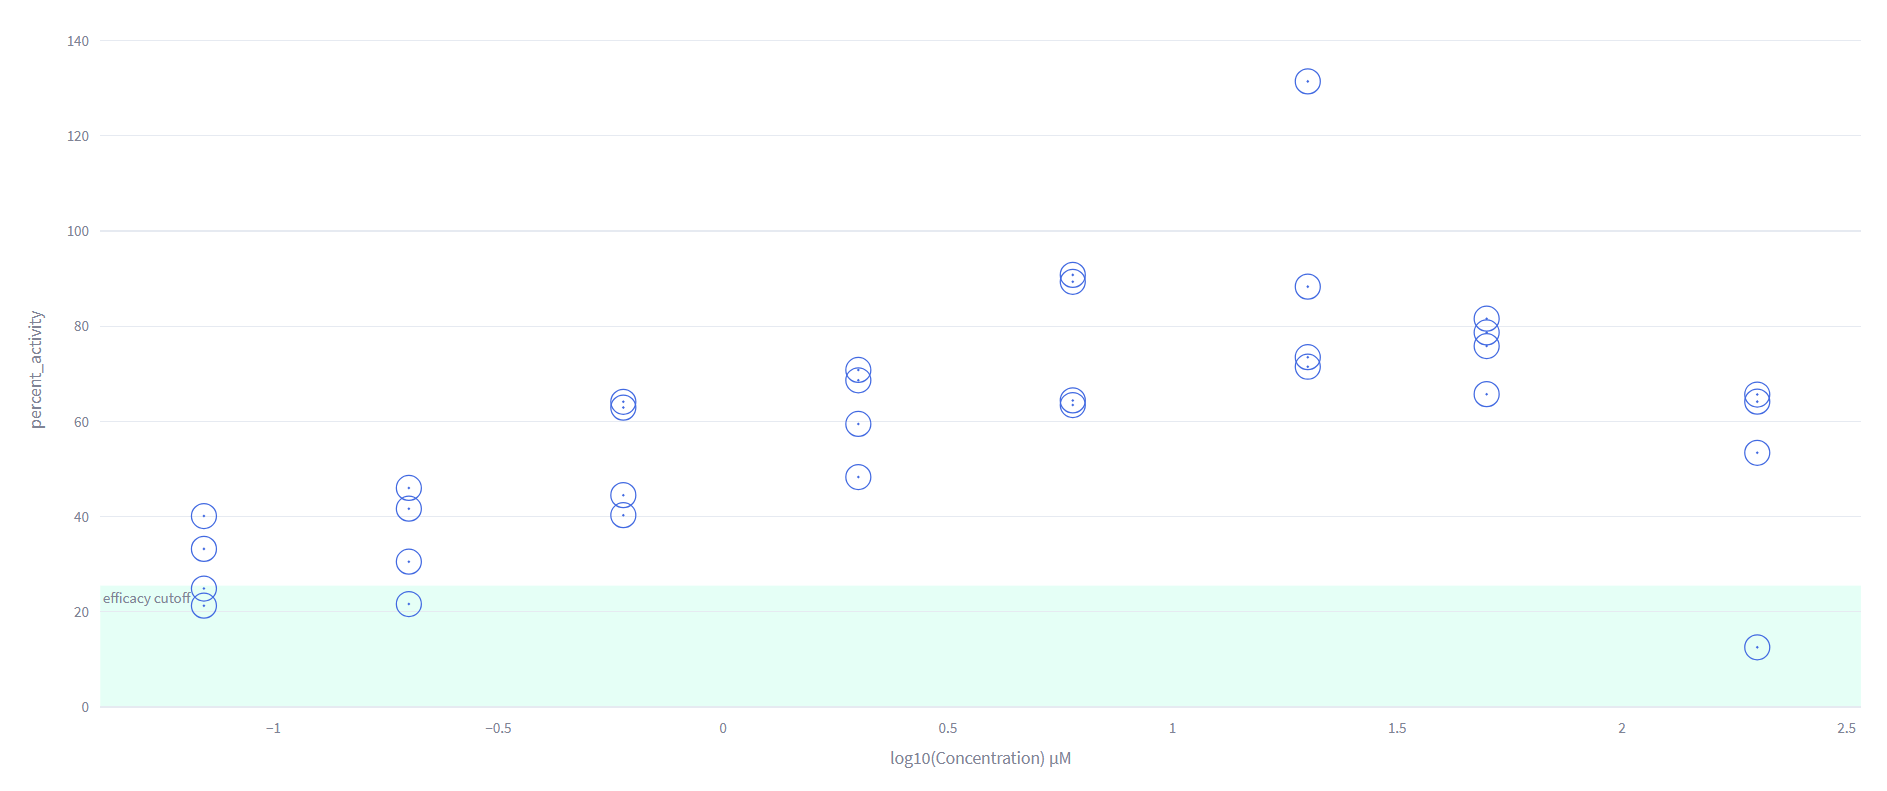
\includegraphics[width=1.0\textwidth]{figures/concentration_response_series.png}  
    \caption{A concentration-response series for the compound \textit{Estropipate} (DTXSID3023005) in the assay endpoint \textit{TOX21\_ERa\_LUC\_VM7\_Agonist} (aeid=788). The series has a total of $k = 45$ concentration-response pairs and is composed of $n_{conc} = 15$ concentration groups, each with $n_{rep} = 3$ replicates.}
~\label{fig:concentration_response_series} 
\end{figure}

In this section, we demonstrate the significance of variations in concentration-response pairs among different compounds and assay endpoints. In practice, concentrations are often subjected to multiple testing iterations, resulting in the formation of distinct concentration groups. Within each concentration group, the number of replicates is indicated by $n_{rep}$.
We introduce the following quantities corresponding to a concentration-response series for a compound $c_i$ in a given assay endpoint $a_i$:
\begin{itemize}
    \item $n_{\text{datapoints}_{i,j}}$: the total number of concentration-response pairs ($|S|$)
    \item $n_{\text{groups}_{i,j}}$: the number of distinct concentrations tested
    \item $n_{\text{replicates}_{i,j}}$: the number of replicates for each concentration group
    \item $min_{\text{conc}_{i,j}}$: the lowest concentration tested
    \item $max_{\text{conc}_{i,j}}$: the highest concentration tested
\end{itemize}


For an overview of these quantities across the entire set of considered concentration-response series, please refer to Figure~\ref{fig:concentration_metric_distributions}. This figure illustrates the above metrics aggregated by their means, grouped by assay endpoints and compounds.



\begin{figure}[htbp]  % Placement options: h (here), t (top), b (bottom), p (page)
    \centering
    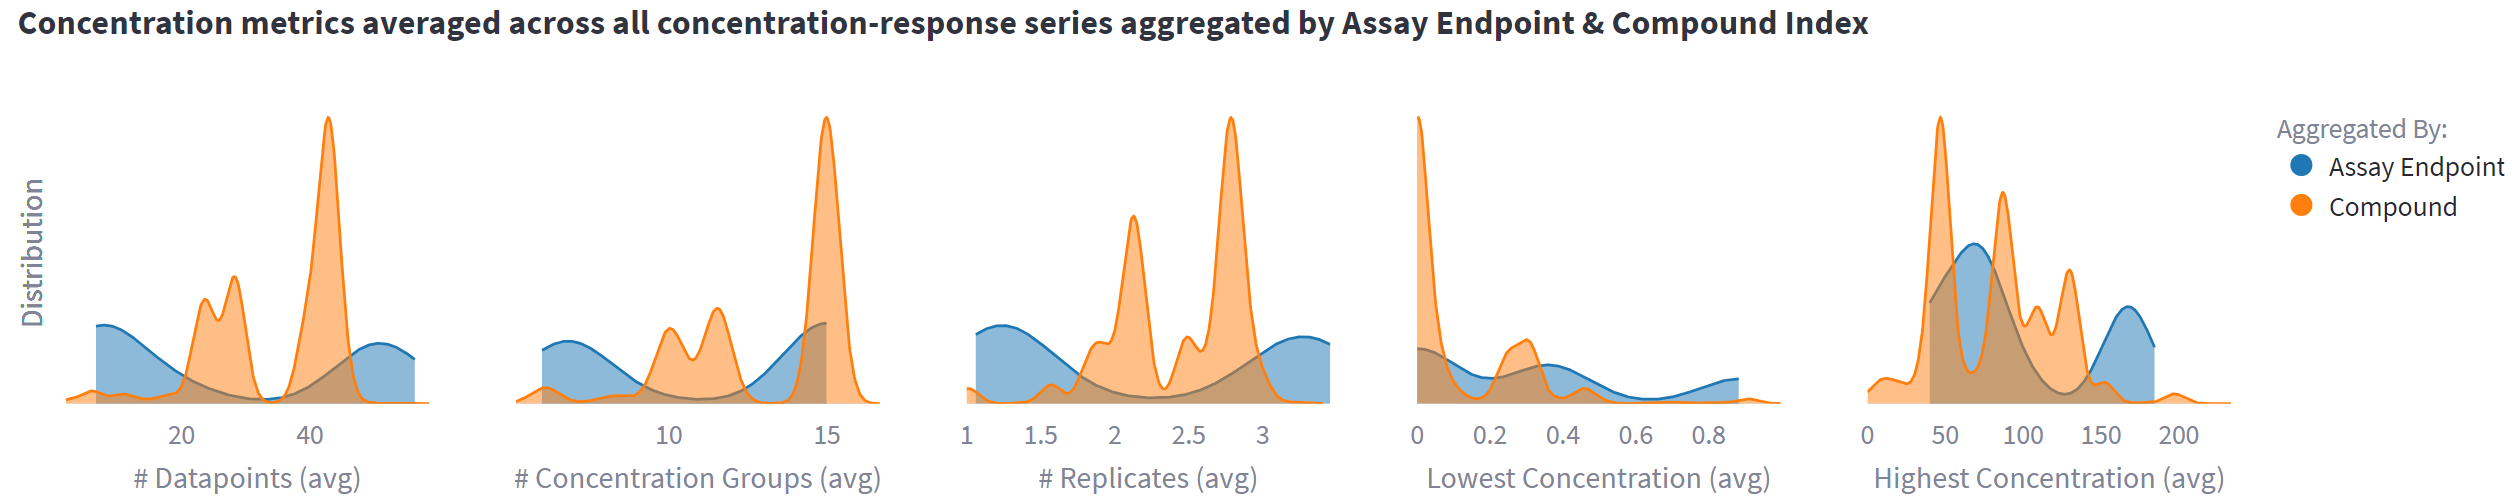
\includegraphics[width=1.0\textwidth]{figures/concentration_metric_distributions.png}  
    \caption{Concentration metrics averaged across all concentration-response series aggregated by assay endpoint (blue) and compound (orange). E.g., the first chart shows the distribution on the average number of datapoints across all assay enpoint $a_i \in A$ with $\frac{1}{|C|} \sum_{j} n_{\text{datapoints}_{i,j}}$ and across all compounds $c_j \in C$ with $\frac{1}{|A|} \sum_{i} n_{\text{datapoints}_{i,j}}$. The same is done for the other metrics: $n_{\text{groups}_{i,j}}$, $n_{\text{replicates}_{i,j}}$, $min_{\text{conc}_{i,j}}$, and $max_{\text{conc}_{i,j}}$.
    }
~\label{fig:concentration_metric_distributions} 
\end{figure}


\section{Pytcpl}
We introduce \href{https://github.com/rbBosshard/pytcpl}{pytcpl}, a streamlined Python package inspired by the R package \href{https://github.com/USEPA/CompTox-ToxCast-tcpl}{tcpl}, designed for processing high-throughput screening data. The package primarily focuses on providing essential features such as concentration-response curve fitting and allows for continuous hit-calling for compound bioactivity across diverse assay endpoints, akin to \href{https://github.com/USEPA/CompTox-ToxCast-tcplFit2}{tcplfit2}. \href{https://cfpub.epa.gov/si/si_public_record_Report.cfm?dirEntryId=355484&Lab=CCTE}{Invitrodb version 3.5 release} can optionally serve as backend database if desired. The package optimizes data storage and provides compressed raw data and metadata from \emph{invitroDB} in Parquet files. This efficient strategy reduces storage needs, resulting in just 4 GB within the repository—compared to the original 80 GB database. This obviates the need for a cumbersome, large-scale database installation, rendering downstream analysis more accessible and efficient. Our package is crafted to accomodate cusomizable processing steps and facilitate interactive data visualization with \href{https://pytcpl.streamlit.app/}{curve surfer}. Moreover, it empowers Python-oriented researchers to seamlessly engage in data analysis and exploration.

\subsection{Pipeline}
\begin{enumerate}
    \item Data collection
    \item Cutoff determination and filtering (Meet conditions for curve fitting)
    \item Curve fitting
    \item Hit calling
\end{enumerate}
\subsubsection{Data Collection}
First, all datapoints are collected from the database and assigned to the concentration response-series belonging to the respective compound in the corresponding assay endpoint.
\subsubsection{Curve Fitting}
Introduce all candidate fit models, discuss the pros and cons of each model. Discuss the fitting procedure, how the models are fitted, Maximum Likelihood Estimation
\subsubsection{Hit Calling}
Akaike criterion, probability of being active, etc..
\subsection{Curve Surfer}
Data visualization, overview of what is possible with the tool. Filter by assay endpoint, compound, etc.


\section{Machine Learning Pipeline}
\subsection{Preprocessing}
Subselecting the columns from the output tables generated by pytcpl: DTXSID identifier and continuous hitcall value. The feature inputs to the machine learning model is a molecular structure represented as fingerprint generated from a SMILES string uniquely determined by the compounds DTXSID identifier. The SMILES string is a linear representation of a compound's molecular structure. The SMILES string is converted to a molecular graph, which is then converted to a feature vector. The feature vector is then used to train a machine learning model. The machine learning model is then used to predict the hitcall value for a given compound. The machine learning pipeline is illustrated in Figure~\ref{fig:ml_pipeline}. 


\subsection{Binary Classification}
The goal is to predict whether a compound is active or inactive for a given assay endpoint. We can formulate this as a binary classification problem, where the input is the compound's molecular structure fingerprint and the output is the hitcall value binarized by some decision threshold. The hitcall value is rendered to a binary variable, where 1 indicates that the compound is active and 0 indicates that the compound is inactive.
\subsection{Regression}
\subsection{Massbank Validation}
